\section{Überblick und Aufbau der bestehenden Ergebnisanzeige}
\label{ch:IST-Zustand:sec:Aufbau_altes_System}

Das System zur Anzeige der Testpoolergebnisse besteht aus verschiedenen Oberflächen, die jeweils einen Anwendungsfall darstellen. \autoref{fig:aufbau_altes_System} ist ein Ausschnitt aus der Oberfläche. Außerhalb des Bildausschnitts sind aufklappbare Menüs (Drop-Down-Menüs) zu finden, in denen die Attribute, wie beispielsweise der Maschinenname und die Versionsnummer, auswählbar sind. Die Oberflächen sind weiterhin über einen internen Link zugänglich, in dem alle Attribute zur Identifikation angegeben sind.

\begin{figure}[H]
    \centering
    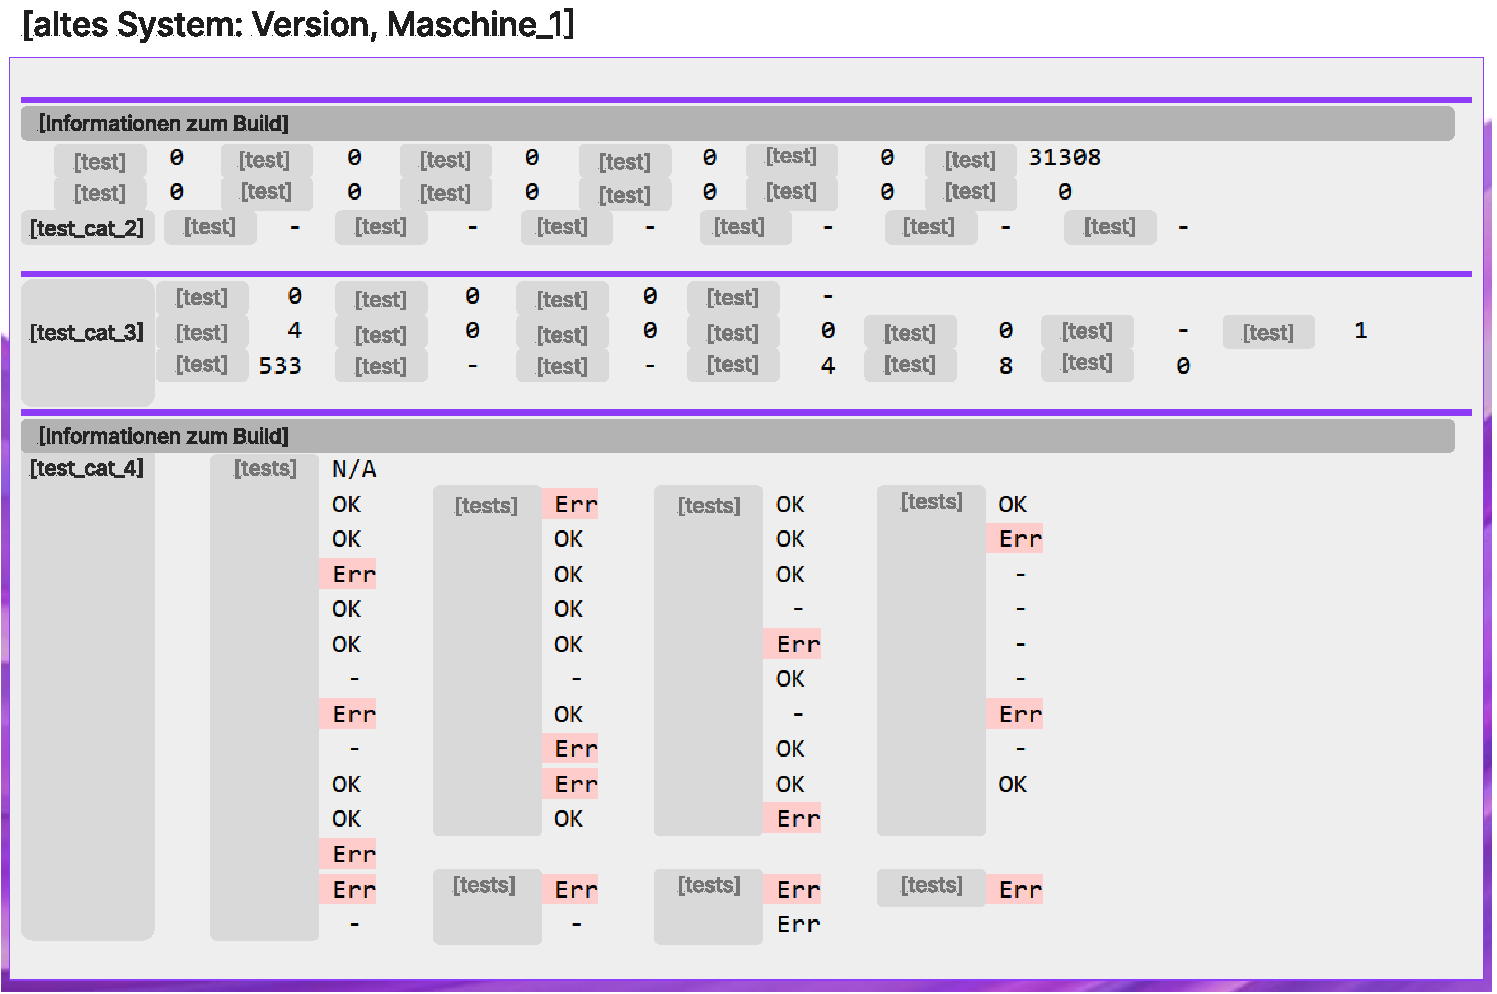
\includegraphics[width=1\linewidth]{Dashboard/altesSystem_zensiert.pdf}
    \caption{Beispielhafter Aufbau einer Oberfläche im alten System}
    \label{fig:aufbau_altes_System}
\end{figure}

\noindent
Der Bildausschnitt von \autoref{fig:aufbau_altes_System} zeigt die Testergebnisse eines Anwendungsfalls. Die Attribute, die diesen Anwendungsfall beschreiben, stehen links, oberhalb der Testergebnisse. Das Bild ist zensiert, damit keine Rückschlüsse auf interne Informationen gezogen werden können, wobei der konkrete Inhalt unabhängig für diese Untersuchung ist.

Im Hauptbereich sind insgesamt drei Reihen mit Textfeldern zu erkennen. Diese lassen sich in die Testfall-Kategorien unterscheiden, wie zum Beispiel \textit{[test\_cat\_2]}. Dieser Kategoriename steht jeweils in der linken Spalte. Die erste dieser Kategorien hat keinen Namen, jedoch werden alle dort aufgeführten Tests mit dem Bauprozess (\textit{Build}) assoziiert. Die dazugehörigen Informationen wie System, Datum, Uhrzeit und Versionsnummer sind an Stelle des Feldes \textit{[Informationen zum Build]} aufgelistet.

Pro Kategorie sind alle Testumgebungen, die jeweils aus einer Sammlung an Tests bestehen, in Spalten aufgelistet. Rechts neben einer Spalte ist das jeweilige zusammengefasste Ergebnis dieser Testsammlung dargestellt. Hierbei zeigen die ersten drei Kategorien die Anzahl der fehlgeschlagenen Testfälle an. Steht ein einfacher Querstrich als Ergebnis, so konnte diese Test\-um\-ge\-bung noch nicht vollständig ausgeführt werden, wodurch noch kein Ergebnis ersichtlich ist. In Test-Kategorie vier wird hingegen der Zustand der Testsammlung angezeigt. Bei \glqq OK\grqq{} sind alle Tests ohne Fehler durchgelaufen. Wird \glqq Err\grqq{} angezeigt, gibt es mindestens einen Test, der fehlgeschlagen ist. Der Querstrich sagt weiterhin aus, dass diese Tests noch nicht gelaufen sind. Eine weitere mögliche Anzeige ist \glqq CORE\grqq{}. Wird dies dargestellt, so ist ein Test abgestürzt und der Prozess muss neu gestartet werden. Der letzte dargestellte Status \glqq N/A\grqq{} steht für not available (dt. nicht verfügbar). Diese Testsammlung findet im angezeigten Kontext keine Anwendung.

%\underline{Auf dem Bild erkennbar (s. \autoref{fig:aufbau_altes_System})}\\
%Name des Kontexts\\
%Build-Infos\\
%Test-Kategorien in Zeilen\\
%Testumgebungen / -namen jeweils in Spalten - den Zeilen zugeordnet\\
%-> zusammengefasstes Testergebnis daneben\\
%--> Test-Kategorie 1,2,3: Anzahl der Fehler als Zahlwert oder Kürzel für 'Absturz im Bauprozess'\\
%--> Test-Kategorie 4: Auflistung des Zustands (Ok, Err (Fehler), - (noch nicht gelaufen) oder Crash)
